\documentclass[a4paper,UTF8]{article}
\usepackage{ctex}
\usepackage[margin=1.25in]{geometry}
\usepackage{color}
\usepackage{graphicx}
\usepackage{amssymb}
\usepackage{amsmath}
\usepackage{amsthm}
%\usepackage[thmmarks, amsmath, thref]{ntheorem}
\theoremstyle{definition}
\newtheorem*{solution}{Solution}
\newtheorem*{prove}{Proof}
\usepackage{multirow}
\usepackage{url}
\usepackage{enumerate}
\usepackage{algorithm}
\usepackage{algorithmic}
\usepackage{caption}
\usepackage{subcaption}
\usepackage{booktabs}
\usepackage{listings}
\renewcommand{\algorithmicrequire}{\textbf{Input:}}
\renewcommand{\algorithmicensure}{\textbf{Procedure:}}
\renewcommand\refname{参考文献}

%--

%--
\begin{document}
\title{实验3. 强化学习实践}
\author{MG1733098,周华平,\url{zhp@smail.nju.edu.cn}}
\maketitle

\section*{综述}


\section*{实验二.}

\subsection*{Q-learning实现}

Q-learning算法采用了$\epsilon$-贪心法,基于一个概率来对探索和利用进行折中。
若尝试次数非常大,那么在一段时间后,Action的Reward都能很好地近似出来,不需要再探索。
因此,对于Q-learning以及之后的DQN,假设当前尝试次数为$t$,
我们使用公式(\ref{eq:eps})来对$\epsilon$进行更新。

\begin{equation}
	\label{eq:eps}
	\epsilon = eps\_end+(eps\_start-eps\_end)*\exp(-t/eps\_decay)
\end{equation}

基于同样的理由,对于learning rate $\alpha$,我们可以采用类似的公式(\ref{eq:alpha})进行更新。

\begin{equation}
	\label{eq:alpha}
	\alpha = lr\_end+(lr\_start-lr\_end)*\exp(-t/lr\_decay)
\end{equation}

在Python中实现Q-learning算法主要利用了numpy提供的一些函数。
我们将Q值函数用Python的dict来表示,
用\lstinline[language=Python]{defaultdict(lambda: np.zeros(action_space.n))}
来对Q table进行初始化。
Q table的key是经过离散化后的状态,value是所有Action对应的Q值构成的ndarray。
这里的defaultdict是Python提供的collections容器,
作用是在调用get时对value进行初始化操作。
我们通过一个lambda表达式将qtable中的所有Q值都初始化为0。
算法其他部分的实现比较直观,基本和伪代码中的结构一一对应,因此这里不过多赘述,
具体实现详见myQLearning.py。

需要特别指出的是,为了加快训练算法的收敛速度,
我对每个任务的Reward进行了简单的重新定义。
具体来说,对于CartPole,当轨迹在某一步提前结束时,该步的Reward为$-100$;
而对于MountainCar和Acrobot,当轨迹在某一步提前结束时,该步的Reward为$100$。
这里的定义利用了一个非常直接的观察:
CartPole需要坚持的越久越好,而MountainCar和Acrobot则越快完成越好。
除此之外,我并没有对状态参数进行额外的分析,从而“凑出”一个更好的Reward,
即使这样得到的训练效果可能会更好。
我认为对于状态参数的分析并不应该由人来完成,
如果Reward被人工定义为关于状态参数的一个复杂函数,
则这个函数包含了我们对于这个任务的一些先验知识,
而这些本应该由算法在训练过程中慢慢学习。
如果利用了这些复杂的先验知识的话,我感觉和在游戏中开外挂没什么区别。

\subsection*{Q-learning训练}

对于Q-learning中的几个任务,
我们统一采用\lstinline[language=Python]{np.linspace()}来对状态空间进行离散化,
具体参数如表\ref{tab:disc-ql}所示。

\begin{table}[H]
	\centering
	\caption{Q-learning离散化参数}\label{tab:disc-ql}
	\begin{tabular}{c|ccc}
		\toprule
		& CartPole & MountainCar & Acrobot \\
		\midrule
		start & $(-2.4, -1.1, -12^\circ, -1.5)$ & $(-1.2, -0.07)$ & $(-1, -1, -1, -1, -4\pi, -9\pi)$ \\
		stop & $(2.4, 1.1, 12^\circ, -1.5)$ & $(0.6, 0.07)$ & $(1, 1, 1, 1, 4\pi, 9\pi)$ \\
		num & $(5, 5, 9, 5)$ & $(20, 20)$ & $(10, 10, 10, 10, 10, 10)$ \\
		\bottomrule
	\end{tabular}
\end{table}

Q-learning的超参数设置如表\ref{tab:arg-ql}所示。

\begin{table}[H]
	\centering
	\caption{Q-learning超参数设置}\label{tab:arg-ql}
	\begin{tabular}{ccccc}
		\toprule
		超参数 & 参数意义 & CartPole & MountainCar & Acrobot \\
		\midrule
		discount & Q-learning算法中的$\gamma$ & 0.99 & 0.99 & 0.9 \\
		lr\_start & $\alpha$的初始值 & 0.9 & 0.9 & 0.9 \\
		lr\_end & $\alpha$的结束值 & 0.001 & 0.0015 & 0.0015 \\
		lr\_decay & $\alpha$的衰减权重 & 1000 & 200 & 200 \\
		eps\_start & $\epsilon$的初始值 & 0.9 & 0.9 & 0.9 \\
		eps\_end & $\epsilon$的结束值 & 0.05 & 0.05 & 0.05\\
		eps\_decay & $\epsilon$的衰减权重 & 1000 & 200 & 200 \\
		\bottomrule
	\end{tabular}
\end{table}

% TODO reward的均值和标准差
对于每个任务,我将多次训练中得到的最好的策略进行测试。
对于CartPole、MountainCar以及Acrobot,我分别测试了100条轨迹,
最终得到reward的均值和标准差如表\ref{tab:reward-ql}所示。

\begin{table}[H]
	\centering
	\caption{Q-learning Average Reward}\label{tab:reward-ql}
	\begin{tabular}{c|ccc}
		\toprule
		& CartPole & MountainCar & Acrobot \\
		\midrule
		$mean \pm std$ &
		$385.29 \pm 69.15$ &
		$-141.68 \pm 22.79$ &
		$-170.70 \pm 37.79$ \\
		\bottomrule
	\end{tabular}
\end{table}

\section*{实验三.}

\subsection*{DQN实现}

DQN在基本的Deep Q-Learning算法的基础上使用了Experience Replay经验池,
通过将训练得到的数据储存起来然后随机采样的方法来降低数据样本的相关性,进而提升了性能。

在本实验中,我选择使用PyTorch来实现DQN。
在定义Q值网络时我使用了MLP,其中网络结构由3层Linear构成;激活函数使用PReLU,
同时在每个隐层中增加Batch Norm来对相应的activation做规范化操作。
DQN中的神经网络和梯度计算的实现主要利用了PyTorch提供的Optimizer以及loss函数。
具体说来,在DQN中我采用\lstinline[language=Python]{optim.Adam}作为优化函数,
用\lstinline[language=Python]{nn.MSELoss()}来计算均方误差。
$\epsilon$的更新同公式(\ref{eq:eps})。
其余的算法实现细节详见myDQN.py。

Q值网络的定义如下所示:

\begin{lstlisting}[language=Python]
class DQN(nn.Module):
    def __init__(self, input_dim, output_dim, hidden_dim):
        super(DQN, self).__init__()
        self.layer1 = nn.Sequential(
            nn.Linear(input_dim, hidden_dim),
            nn.BatchNorm1d(hidden_dim),
            nn.PReLU(),
        )
        self.layer2 = nn.Sequential(
            nn.Linear(hidden_dim, hidden_dim),
            nn.BatchNorm1d(hidden_dim),
            nn.PReLU(),
        )
        self.out = nn.Linear(hidden_dim, output_dim)

    def forward(self, x):
        x = self.layer1(x)
        x = self.layer2(x)
        return self.out(x)
\end{lstlisting}

\subsection*{DQN训练}

DQN的超参数设置如表\ref{tab:arg-dqn}所示。

\begin{table}[H]
	\centering
	\caption{DQN超参数设置}\label{tab:arg-dqn}
	\begin{tabular}{ccccc}
		\toprule
		超参数 & 参数意义 & CartPole & MountainCar & Acrobot \\
		\midrule
		memory\_size & Replay Memory的大小 & 10000 & 10000 & 5000 \\
		batch\_size & mini-batch的大小 & 128 & 128 & 128 \\
		hidden\_dim & DQN的隐层维度 & 50 & 50 & 50\\
		discount & DQN算法中的$\gamma$ & 0.99 & 0.99 & 0.99 \\
		learning\_rate & DQN算法中的$\alpha$ & 0.001 & 0.001 & 0.001 \\
		eps\_start & $\epsilon$的初始值 & 0.9 & 0.9 & 0.9 \\
		eps\_end & $\epsilon$的结束值 & 0.05 & 0.05 & 0.05\\
		eps\_decay & $\epsilon$的衰减权重 & 200 & 50 & 200 \\
		\bottomrule
	\end{tabular}
\end{table}

DQN在CartPole上的实验结果如图\ref{fig:pole-dqn}所示。
%TODO 说明图中的信息
可以观察到Loss在超过450轮后达到收敛的状态。
由于$\epsilon$的最小值被设置为0.05,因此即使Training了较多轮数,
DQN依旧会以5\%的概率随机选择Action。
而CartPole似乎对于错误的Action比较敏感,
当随机到错误的Action时,可能会导致该轨迹提前结束。
因此在Training阶段Reward似乎并没有收敛到一个固定值,
然而我们可以观察到随着Training轮数的增加,
Reward的上限也在不断提高,这也从侧面体现出了训练是有效果的。

\begin{figure}[H]
	\centering
	\begin{subfigure}[t]{0.5\textwidth}
		\centering
		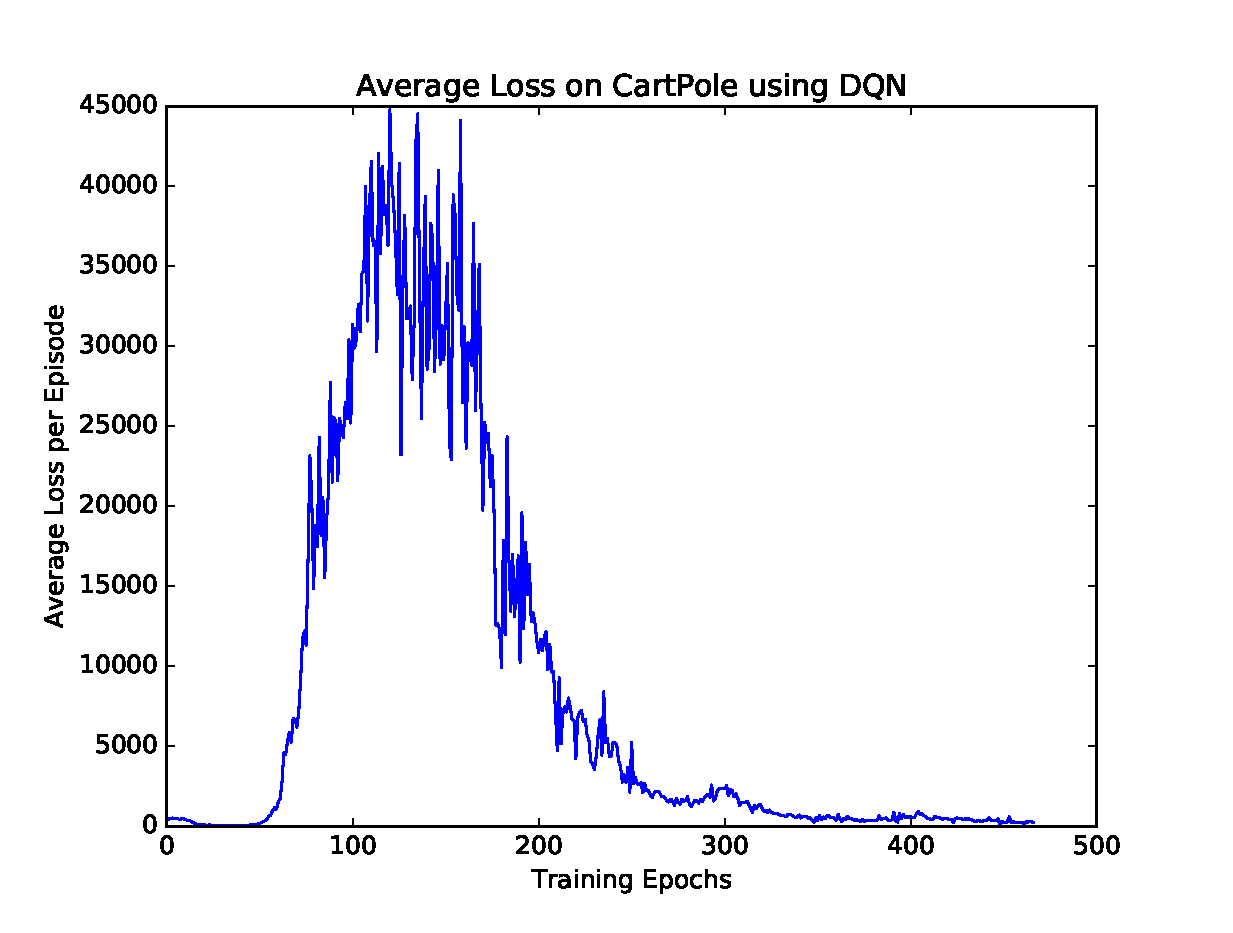
\includegraphics[scale=0.35]{figures/pole-dqn-loss}
		\caption{Average Loss}
	\end{subfigure}%
	\begin{subfigure}[t]{0.5\textwidth}
		\centering
		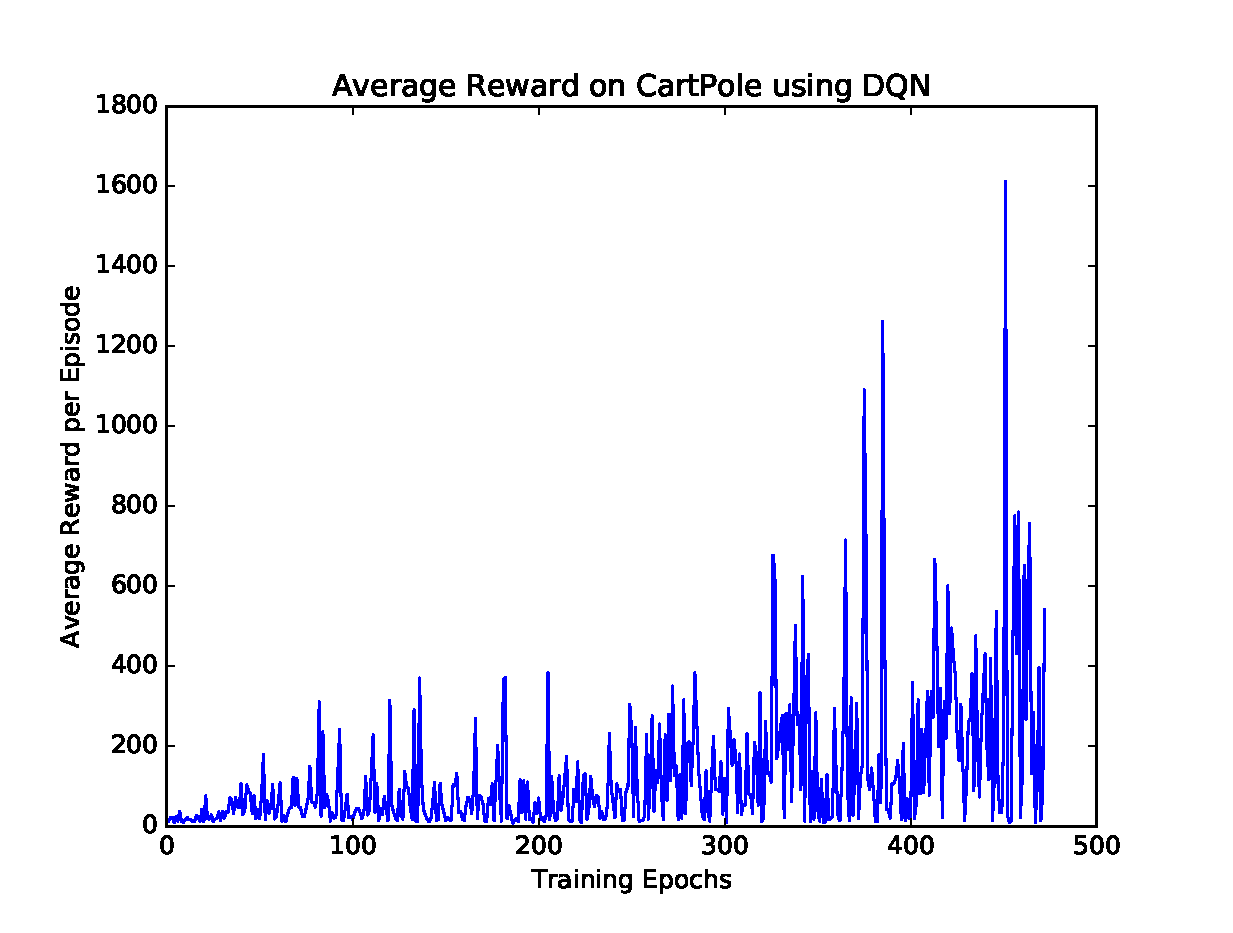
\includegraphics[scale=0.35]{figures/pole-dqn-reward}
		\caption{Average Reward}
	\end{subfigure}
	\caption{Training Result of CartPole using DQN}\label{fig:pole-dqn}
\end{figure}

DQN在MountainCar上的实验结果如图\ref{fig:car-dqn}所示。
其中Reward在超过200轮之后达到收敛的状态,
而Loss也在超过200轮之后达到了基本稳定的状态。

\begin{figure}[H]
	\centering
	\begin{subfigure}[t]{0.5\textwidth}
		\centering
		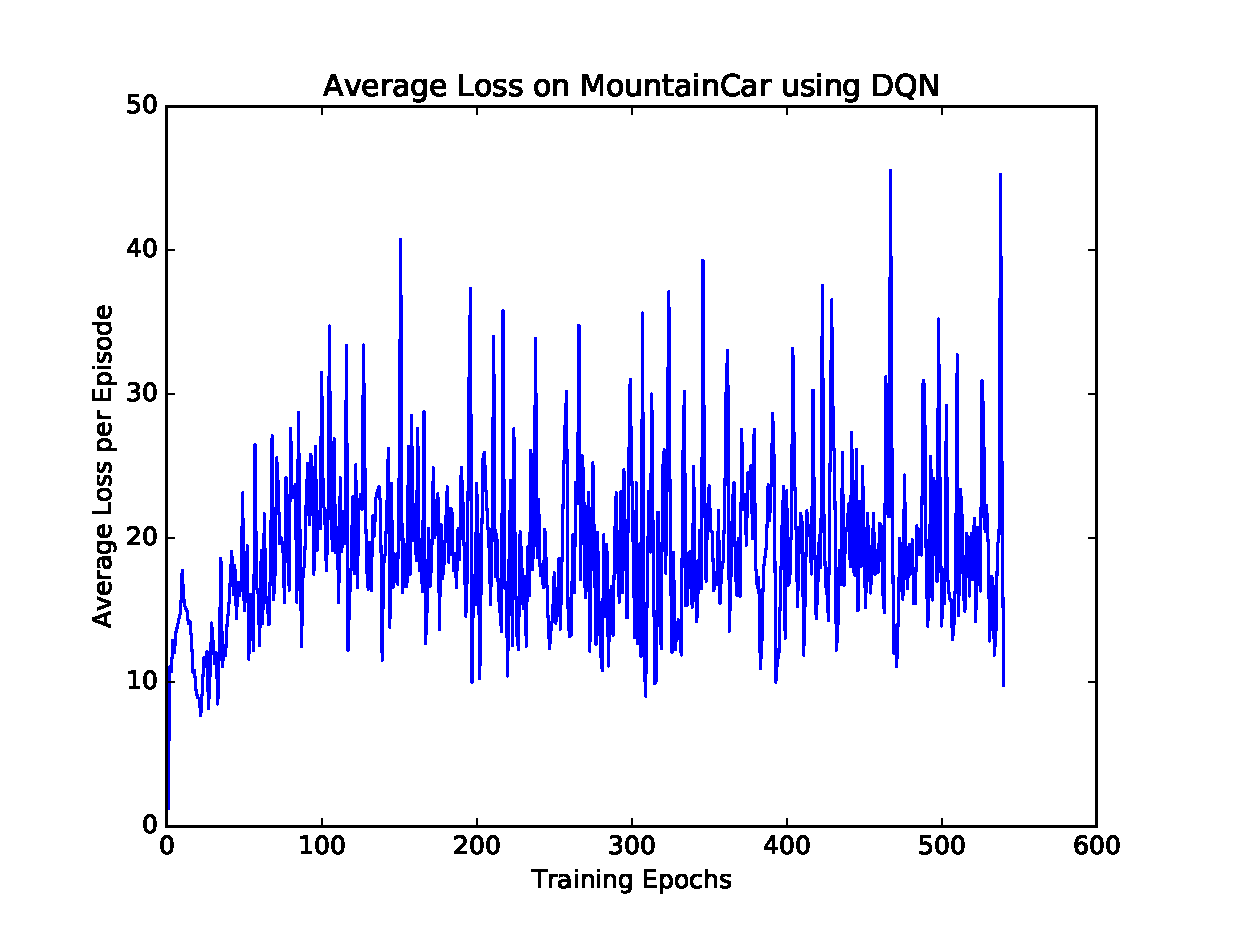
\includegraphics[scale=0.35]{figures/car-dqn-loss}
		\caption{Average Loss}
	\end{subfigure}%
	\begin{subfigure}[t]{0.5\textwidth}
		\centering
		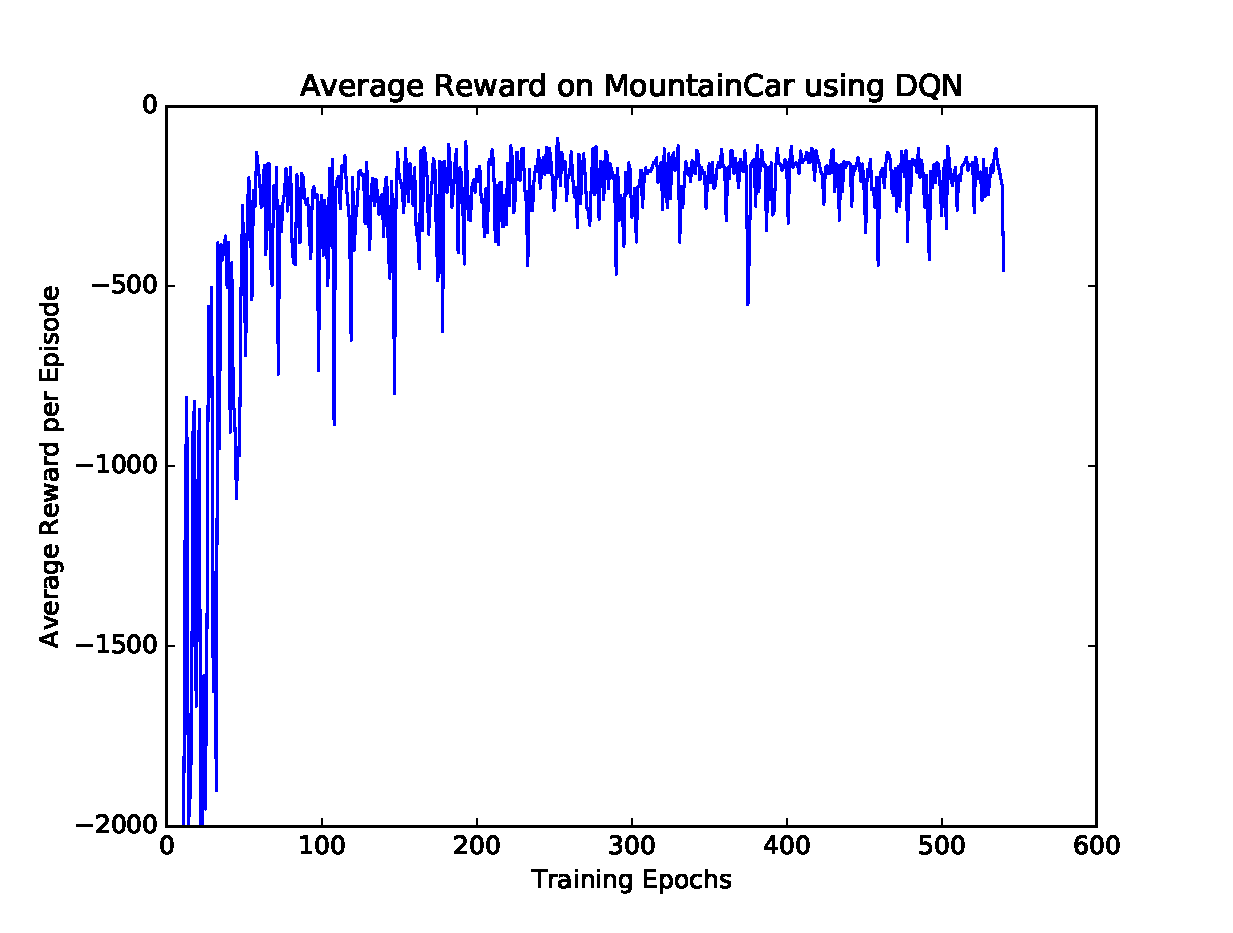
\includegraphics[scale=0.35]{figures/car-dqn-reward}
		\caption{Average Reward}
	\end{subfigure}
	\caption{Training Result of MountainCar using DQN}\label{fig:car-dqn}
\end{figure}

DQN在Acrobot上的实验结果如图\ref{fig:bot-dqn}所示。
在超过40轮之后,Loss达到了较低的水平,并且Reward也趋近于收敛。

\begin{figure}[H]
	\centering
	\begin{subfigure}[t]{0.5\textwidth}
		\centering
		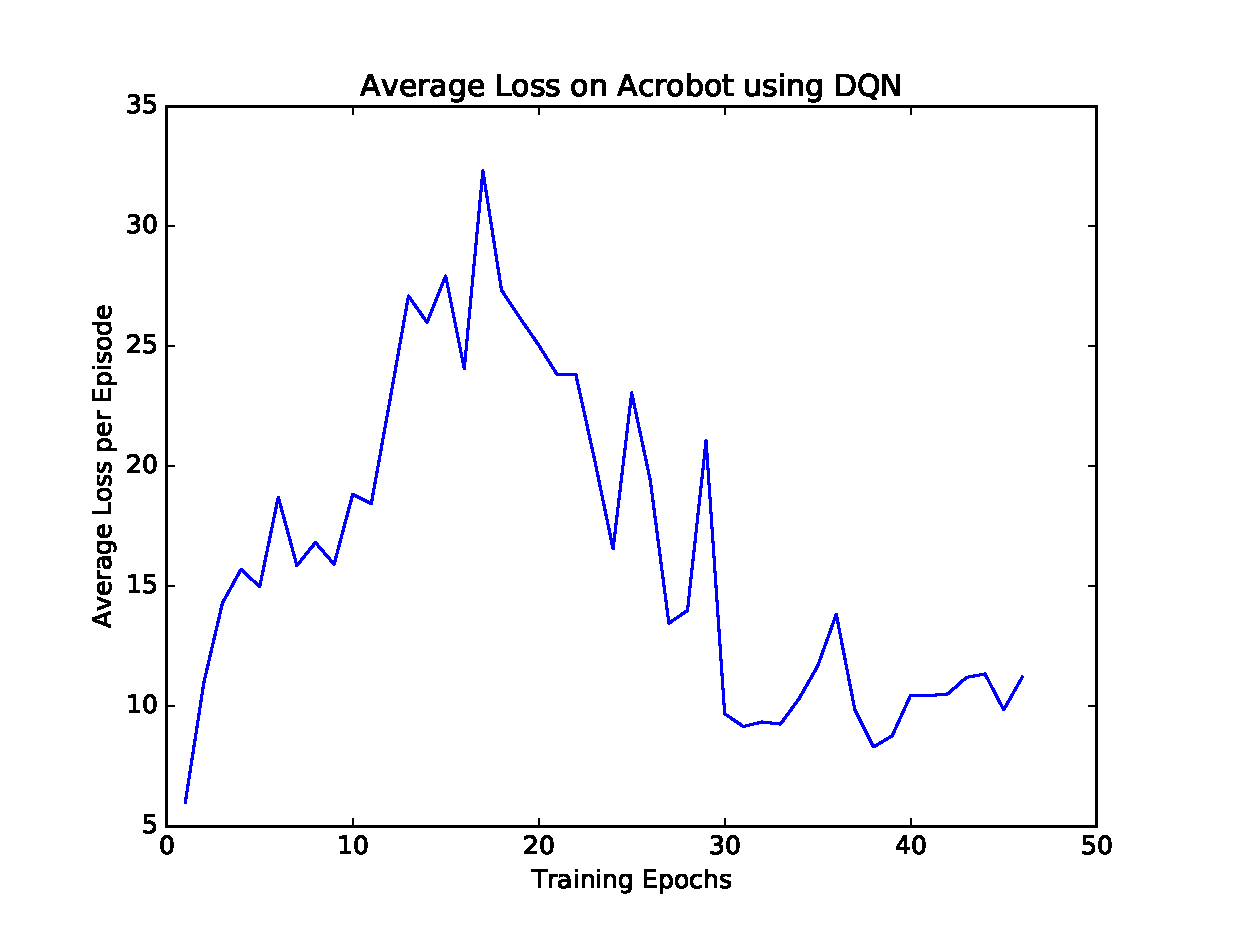
\includegraphics[scale=0.35]{figures/bot-dqn-loss}
		\caption{Average Loss}
	\end{subfigure}%
	\begin{subfigure}[t]{0.5\textwidth}
		\centering
		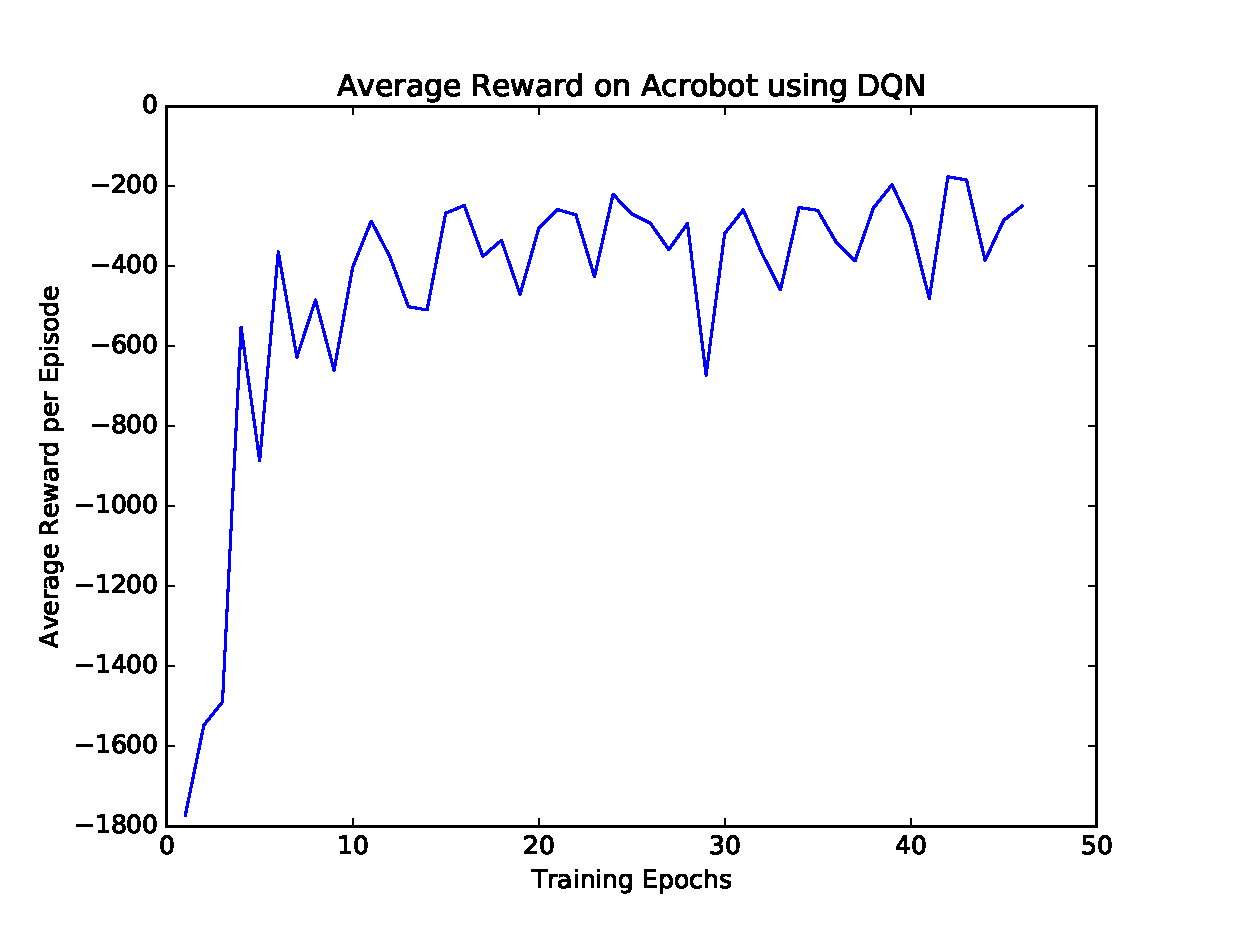
\includegraphics[scale=0.35]{figures/bot-dqn-reward}
		\caption{Average Reward}
	\end{subfigure}
	\caption{Training Result of Acrobot using DQN}\label{fig:bot-dqn}
\end{figure}

对于每个任务,我将多次训练中得到的最好的策略进行测试。
对于CartPole我测试了50条轨迹,
对于MountainCar和Acrobot我分别测试了100条轨迹。
最终得到reward的均值和标准差如表\ref{tab:reward-dqn}所示。

\begin{table}[H]
	\centering
	\caption{DQN Average Reward}\label{tab:reward-dqn}
	\begin{tabular}{c|ccc}
		\toprule
		& CartPole & MountainCar & Acrobot \\
		\midrule
		$mean \pm std$ & $20000 \pm 0$ & $-183.44 \pm 26.6669533318$ & $-86.84 \pm 18.1117199625$ \\
		\bottomrule
	\end{tabular}
\end{table}

\section*{实验四.}

\subsection*{Improved DQN实现}

相比于DQN,Improved DQN进行了一个微小的改动:增加了目标Q网络$\hat{Q}$。
在计算目标Q值时,我们使用专门的目标Q网络$\hat{Q}$来计算,而不是直接使用预更新的Q网络$Q$。
这样做的目的是为了减少目标计算与当前值的相关性。

在DQN中,目标Q网络会随着$Q$的更新而动态变化,这样不利于计算目标Q值,
导致目标Q值和当前的Q值相关性较大,因此Improved DQN提出单独使用一个目标Q网络。
而$\hat{Q}$中的参数是通过延迟更新的方式从$Q$中获得:
在每训练了$C$步之后,Improved DQN将当前$Q$的参数值复制给$\hat{Q}$。

Improved DQN的实现基于DQN,因此代码部分的改动比较少。
另外在Improved DQN中需要新增一个超参数target\_c,用以表示$\hat{Q}$的更新频率。

\subsection*{Improved DQN训练}

Improved DQN的超参数设置如表\ref{tab:arg-idqn}所示。

\begin{table}[H]
	\centering
	\caption{Improved DQN超参数设置}\label{tab:arg-idqn}
	\begin{tabular}{ccccc}
		\toprule
		超参数 & 参数意义 & CartPole & MountainCar & Acrobot \\
		\midrule
		memory\_size & Replay Memory的大小 & 10000 & 10000 & 10000 \\
		batch\_size & mini-batch的大小 & 128 & 128 & 128 \\
		hidden\_dim & DQN的隐层维度 & 50 & 50 & 50 \\
		target\_c & $\hat{Q}$的更新频率 & 10 & 10 & 5 \\
		discount & DQN算法中的$\gamma$ & 0.99 & 0.99 & 0.99 \\
		learning\_rate & DQN算法中的$\alpha$ & 0.001 & 0.001 & 0.001 \\
		eps\_start & $\epsilon$的初始值 & 0.9 & 0.9 & 0.9 \\
		eps\_end & $\epsilon$的结束值 & 0.05 & 0.05 & 0.05 \\
		eps\_decay & $\epsilon$的衰减权重 & 200 & 50 & 200 \\
		\bottomrule
	\end{tabular}
\end{table}

Improved DQN在CartPole上的实验结果如图\ref{fig:pole-idqn}所示。
可以观察到Loss在超过300轮后达到收敛的状态。

\begin{figure}[H]
	\centering
	\begin{subfigure}[t]{0.5\textwidth}
		\centering
		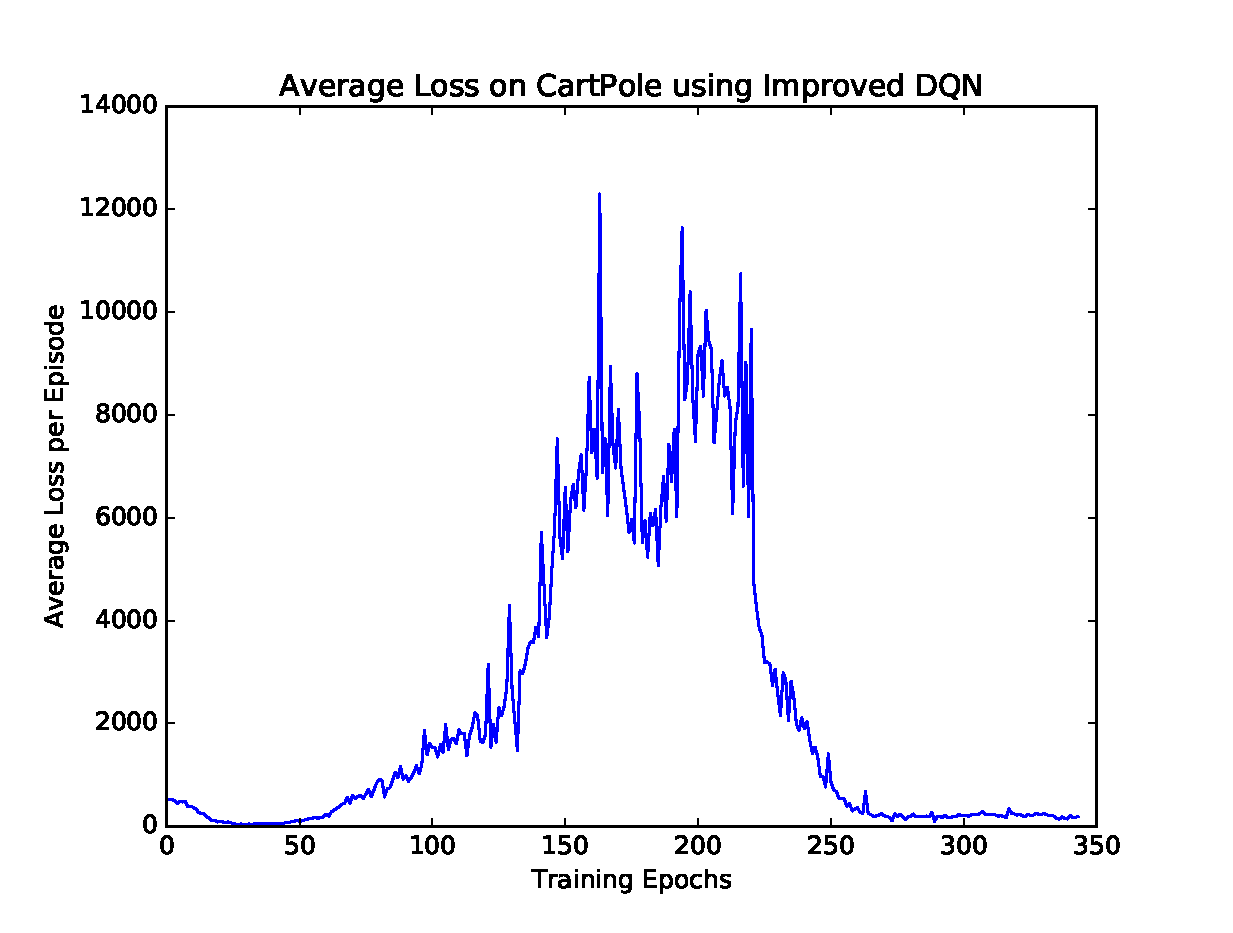
\includegraphics[scale=0.35]{figures/pole-idqn-loss}
		\caption{Average Loss}
	\end{subfigure}%
	\begin{subfigure}[t]{0.5\textwidth}
		\centering
		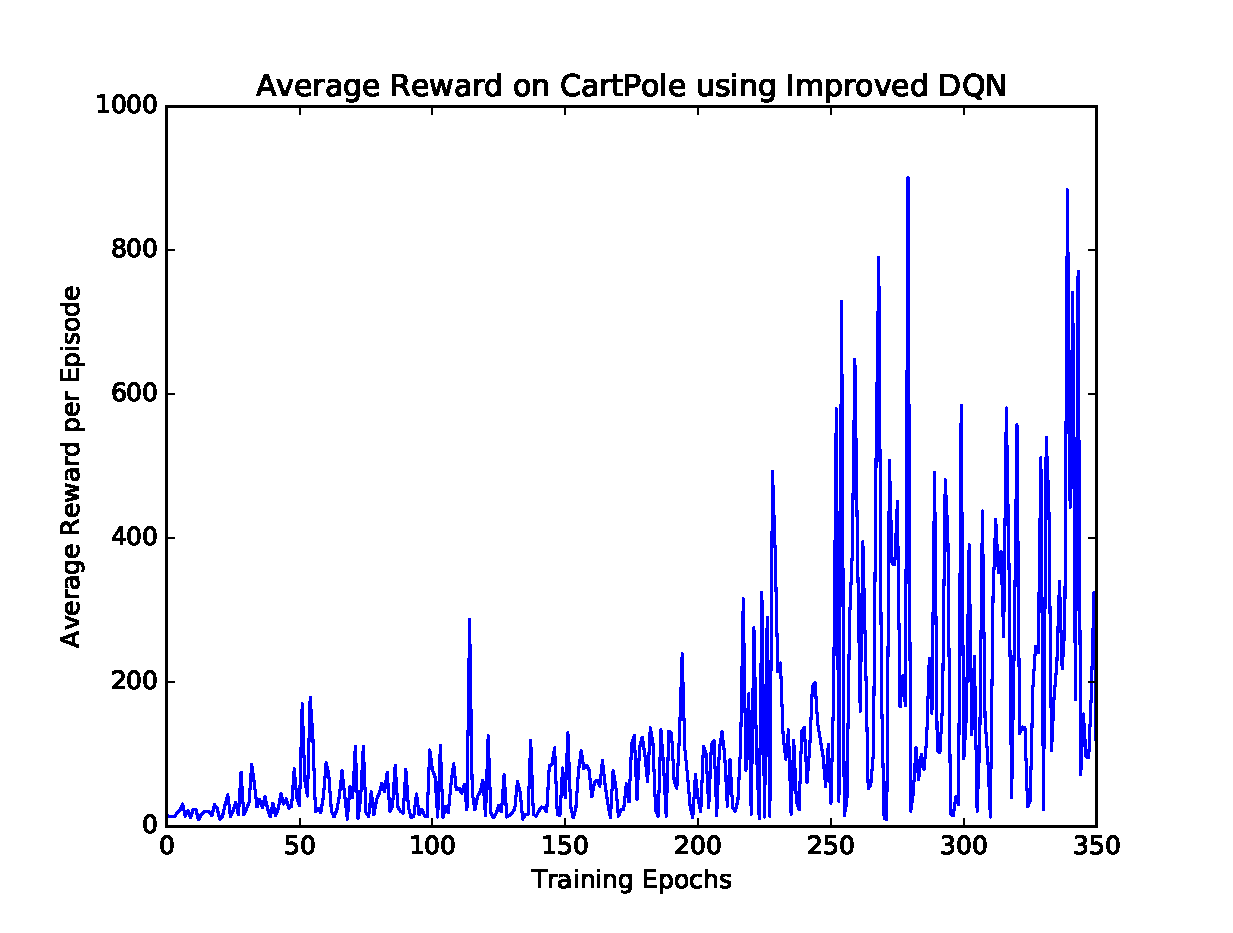
\includegraphics[scale=0.35]{figures/pole-idqn-reward}
		\caption{Average Reward}
	\end{subfigure}
	\caption{Training Result of CartPole using Improved DQN}\label{fig:pole-idqn}
\end{figure}

Improved DQN在MountainCar上的实验结果如图\ref{fig:car-idqn}所示。
其中Reward在超过60轮之后达到收敛的状态,
而Loss也在超过60轮之后达到了基本稳定的状态。

\begin{figure}[H]
	\centering
	\begin{subfigure}[t]{0.5\textwidth}
		\centering
		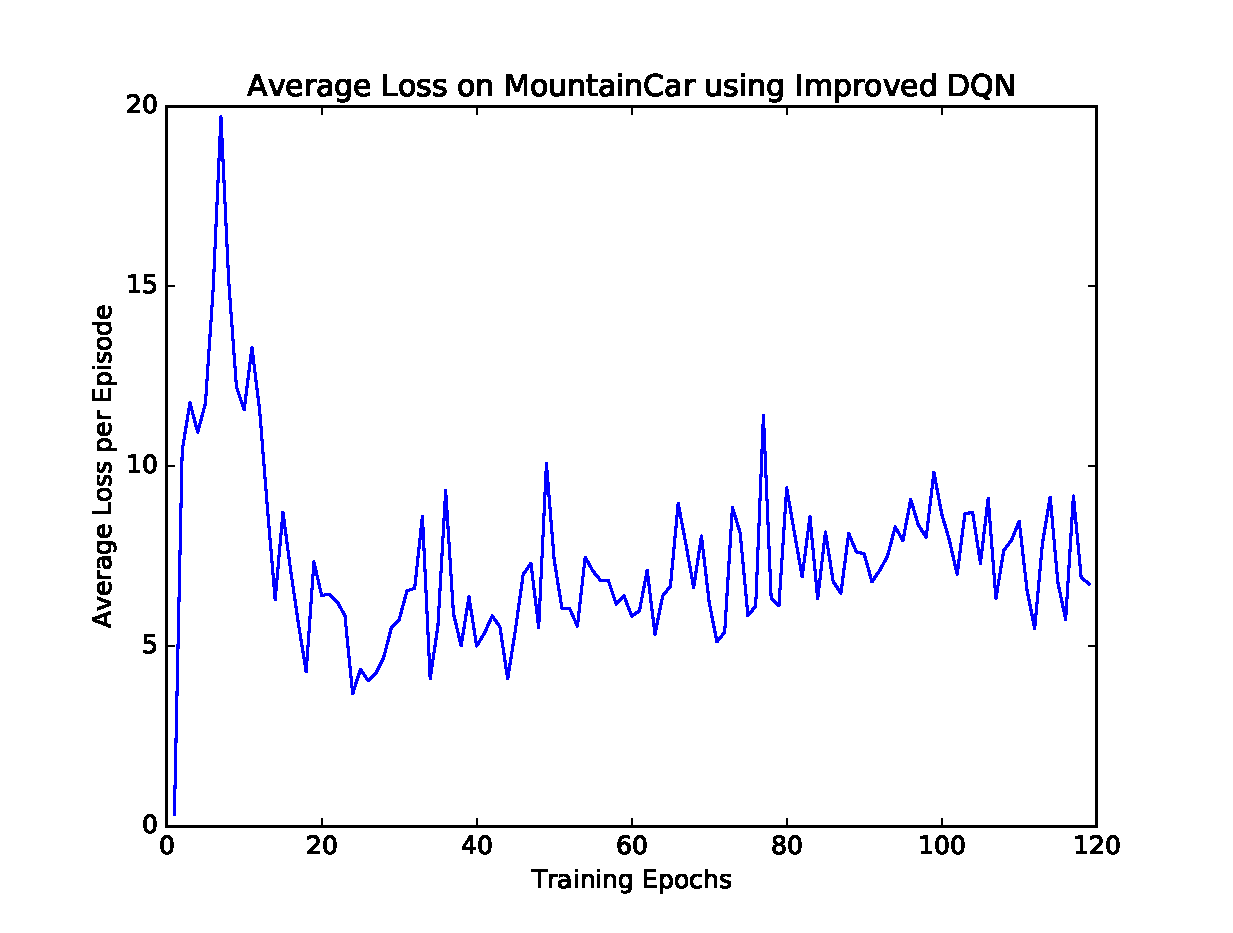
\includegraphics[scale=0.35]{figures/car-idqn-loss}
		\caption{Average Loss}
	\end{subfigure}%
	\begin{subfigure}[t]{0.5\textwidth}
		\centering
		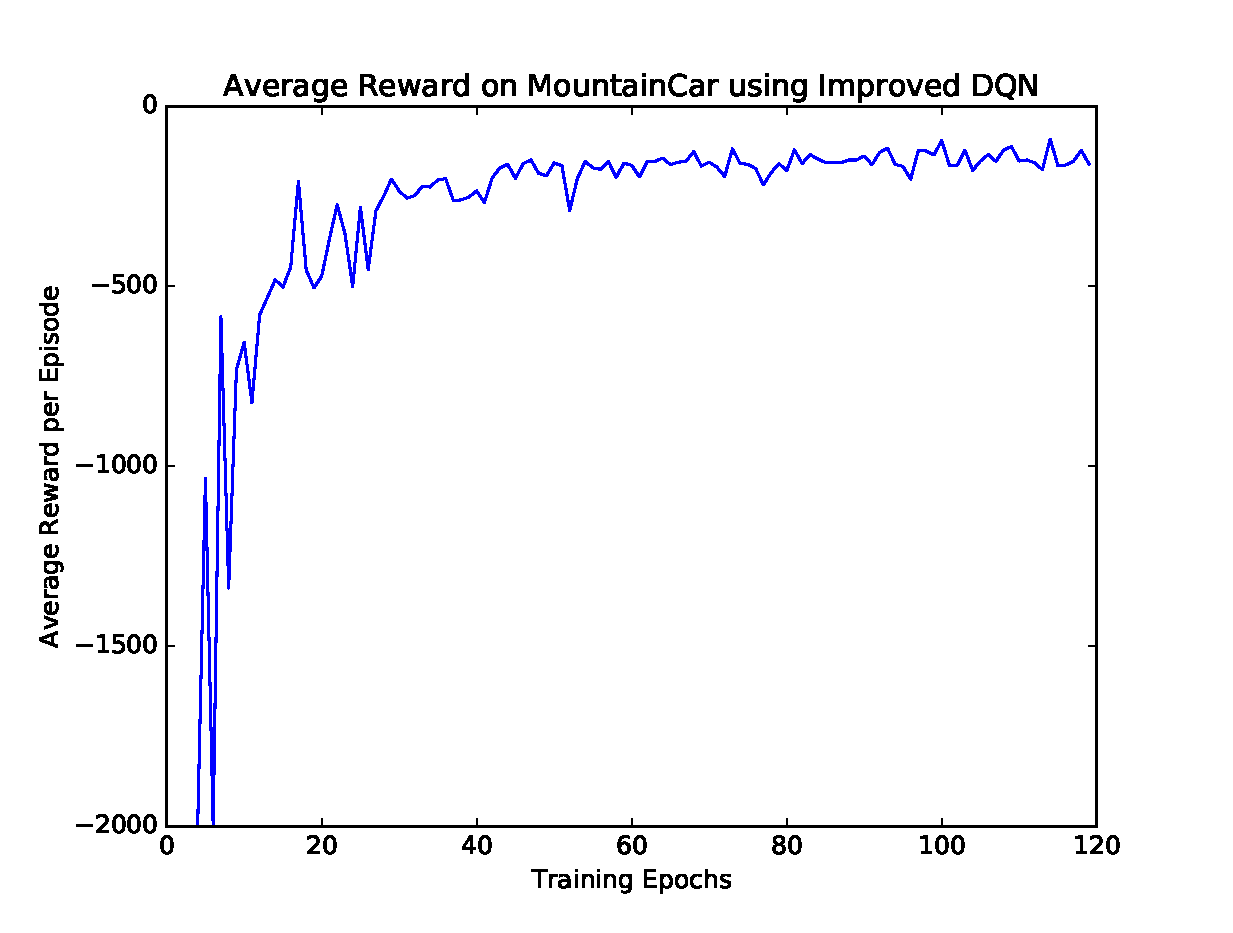
\includegraphics[scale=0.35]{figures/car-idqn-reward}
		\caption{Average Reward}
	\end{subfigure}
	\caption{Training Result of MountainCar using Improved DQN}\label{fig:car-idqn}
\end{figure}

Improved DQN在Acrobot上的实验结果如图\ref{fig:bot-idqn}所示。
在超过50轮之后,Loss达到了较低的水平,并且Reward也趋近于收敛。

\begin{figure}[H]
	\centering
	\begin{subfigure}[t]{0.5\textwidth}
		\centering
		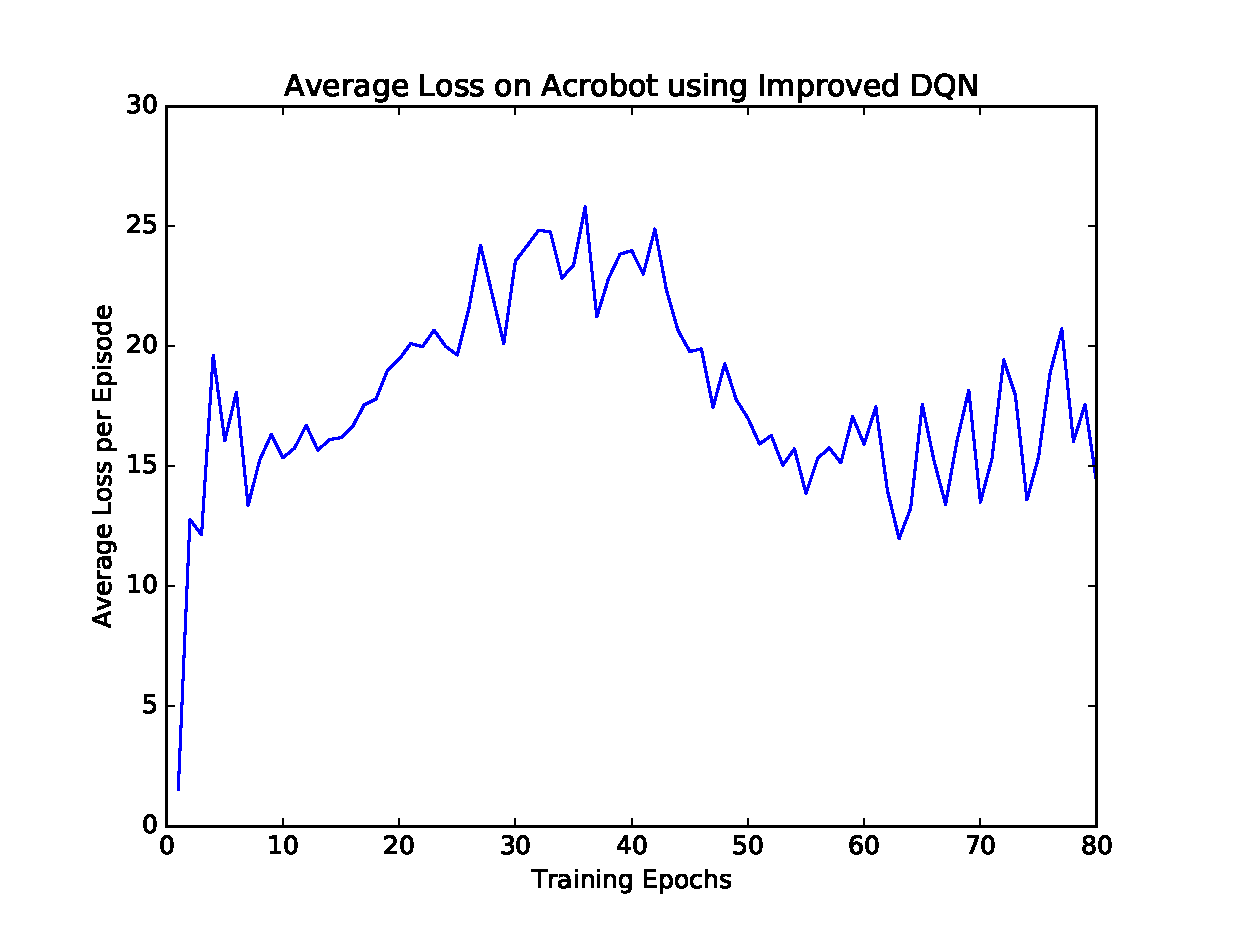
\includegraphics[scale=0.35]{figures/bot-idqn-loss}
		\caption{Average Loss}
	\end{subfigure}%
	\begin{subfigure}[t]{0.5\textwidth}
		\centering
		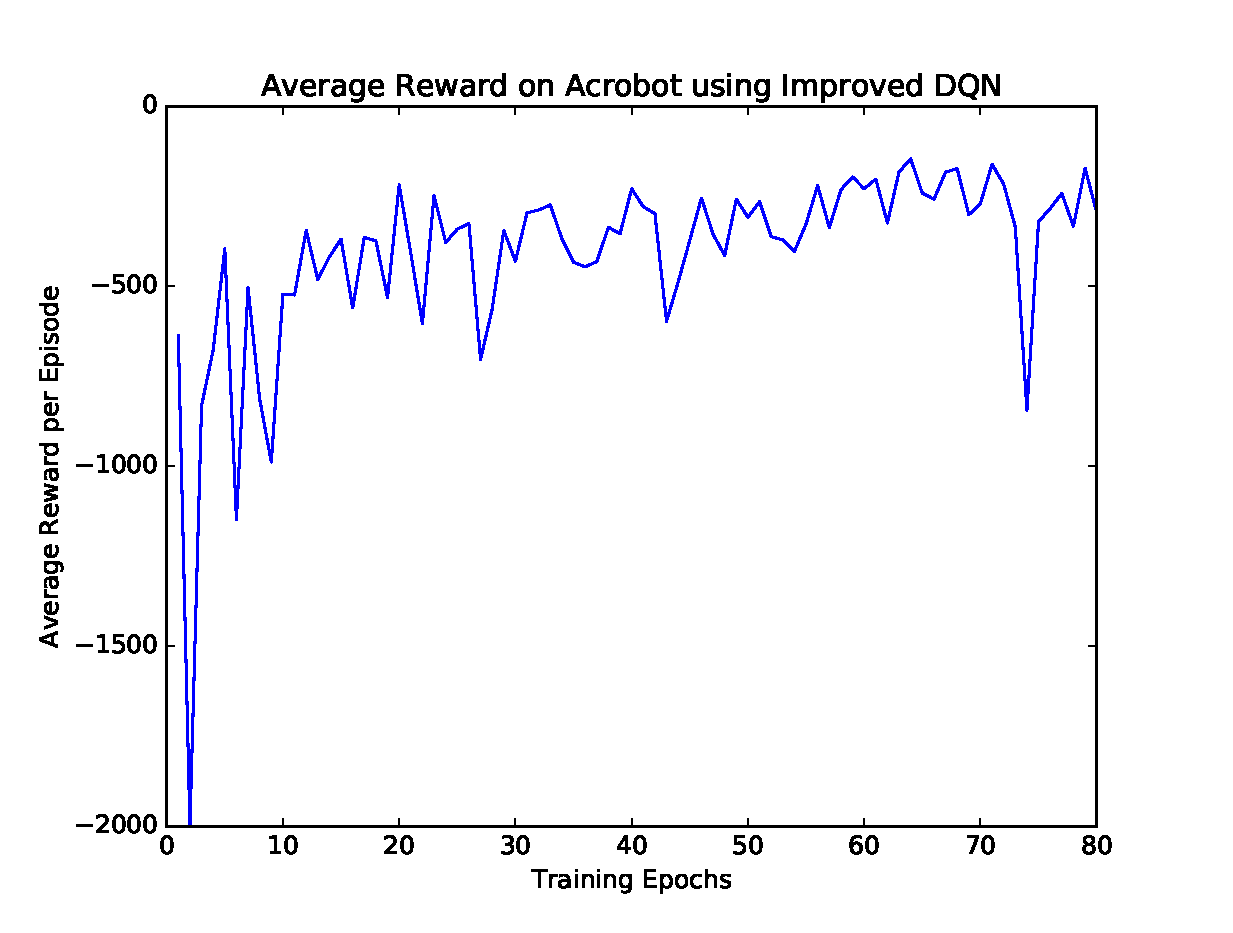
\includegraphics[scale=0.35]{figures/bot-idqn-reward}
		\caption{Average Reward}
	\end{subfigure}
	\caption{Training Result of Acrobot using Improved DQN}\label{fig:bot-idqn}
\end{figure}

对于每个任务,我将多次训练中得到的最好的策略进行测试。
对于CartPole我测试了50条轨迹,
对于MountainCar和Acrobot我分别测试了100条轨迹。
最终得到reward的均值和标准差如表\ref{tab:reward-idqn}所示。

\begin{table}[H]
	\centering
	\caption{Improved DQN Average Reward}\label{tab:reward-idqn}
	\begin{tabular}{c|ccc}
		\toprule
		& CartPole & MountainCar & Acrobot \\
		\midrule
		$mean \pm std$ & $20000 \pm 0$ & $-107.54 \pm 13.5273205033$ & $-84.31 \pm 18.8024971746$ \\
		\bottomrule
	\end{tabular}
\end{table}

\subsection*{Improved DQN与DQN的异同}

在训练过程中可以明显观察到Improved DQN相比于DQN表现得更加稳定,收敛速度也更快。
以MountainCar为例,在使用DQN时,很多时候并没有办法训练出一个可行的模型:
经过几十轮的训练,每一轮的Reward依旧为-2000。
而在前一节中得到的DQN在MountainCar上的比较好的训练结果似乎带有一定的偶然成分;
相比之下,Improved DQN在MountainCar上几乎每次都能训练出一个可行的模型:
在前十轮的训练中,Reward就能突破-2000,并且一旦突破了-2000以后,
Reward能够在之后的每一轮训练中快速增加,直至收敛。

在训练效果上,除了MountainCar以外,
DQN和Improved DQN在CartPole和Acrobot上的训练效果比较接近。
而DQN之所以在MountainCar上的训练结果与Improved DQN差别较大,
我认为主要是由于DQN训练出稳定的MountainCar模型比较困难:
如果能够用DQN训练足够多的模型,
其中最好的那个模型的效果应该和Improved DQN上得到的结果相近。

所以我认为Improved DQN在训练阶段比DQN表现得更加稳定,收敛速度也更快;
而在训练模型收敛后,我猜测DQN与Improved DQN的训练效果应该会比较接近。

\end{document}
